\documentclass[11pt,a4paper]{article}
\usepackage{tikz}
\usetikzlibrary{arrows.meta,positioning}
\usepackage{tabularx}
\usepackage{amsmath,amssymb,amsthm}
\usepackage{geometry}
\geometry{margin=1in}
\usepackage{hyperref}
\usepackage{graphicx}
\usepackage{setspace}
\onehalfspacing

\title{\textbf{Paper D-12: Immune System:\\ A Constraint-Driven Flux Dynamics (CDFD) Perspective}}
\author{Steve Bico Mujjabi, MD\\
\small Independent Researcher\\
\small Founder, Vura Labs\\
\small Kampala, Uganda\\
\small ORCID: 0009-0001-0556-5516}
\date{August 2026}

\begin{document}
\maketitle

% BEGIN SHARED-METHODS POINTER
\noindent\textit{Shared Part IV notation and evidence boundaries are defined in \path{PART_IV_METHODS_AND_CLAIM_BOUNDARY.md}. This paper states only its local observables, comparison, and failure conditions.}
% END SHARED-METHODS POINTER


\begin{abstract}
This paper develops a falsifiable CDFD/AFL model of Immune System. It maps antigen, inflammatory signals, tissue damage, and metabolic demand to driving flux $\Phi$, immune, tissue, vascular, and metabolic capacity to active constraint $C$, regulation, clearance, tolerance, repair, and memory response to responsiveness $S$, and immune memory, scarring, chronic activation, and exposure history to structural memory $M_s$. The target outcome is clearance, protection, collateral damage, and recovery, tested against immune profiling, clinical trajectories, perturbation, pathology, and longitudinal cohorts. The paper treats universality as a shared model architecture rather than an assertion that unlike systems have the same material mechanism. It states the negative result that would make the mapping unnecessary and places the domain claim inside the cumulative CDFD programme and its reproducible runtime boundary.
\end{abstract}

\section{Introduction}

A healthy biological organism must maintain strict boundaries to preserve its internal thermodynamic homeostasis. When pathogens breach these boundaries, they hijack the host's metabolic throughput to replicate, essentially creating an unauthorized, parasitic flow of resources. The immune system's primary function is to detect this parasitic flow and aggressively deploy constraints to halt it.

The CDFD framework posits that all living systems operate under Adaptive Flux Limitation (AFL). The immune response is the ultimate manifestation of AFL: it is the biological mechanism by which the host dynamically manipulates its own internal constraints $C$ to counter external perturbations in $\Phi$.

\section{Immunological Adaptive Flux}
We assess the immunological health of the host via the Adaptive Operating Ratio:
\begin{equation}
    \Psi_s = \left( \frac{\Phi}{C} \right) \cdot S \cdot M_s
\end{equation}

In the context of infection:
\begin{itemize}
    \item \textbf{Flux ($\Phi$)}: The replication rate and pathogenic load of the invading organism (e.g., viral titer), combined with the metabolic toll it exacts on the host.
    \item \textbf{Constraint ($C$)}: The targeted immune response. Cytokines, macrophages, T-cells, and antibodies act to bottleneck and neutralize the pathogenic flux.
    \item \textbf{Responsiveness ($S$)}: The functional capacity of the bone marrow, thymus, and lymphatic system to mobilize a defense without exhausting the host's total energetic budget.
    \item \textbf{Memory ($M_s$)}: Immunological memory (B and T memory cells). Memory ensures that if the same flux profile (antigen) is detected again, the system can instantly deploy massive constraints without a lag phase.
\end{itemize}

\subsection{Cytokine Storms and Autoimmunity}
In a healthy response to infection, the host detects a spike in pathogenic $\Phi$ and proportionally increases $C$ (inflammation) to neutralize it. Once $\Phi$ drops to zero, the constraint $C$ must also relax to restore $\Psi_s \approx 1$ for normal tissue function.

However, if the regulatory feedback loop fails, the system enters a pathological regime. In a \textbf{cytokine storm}, the host overestimates the required constraint, causing $C$ to skyrocket out of proportion to $\Phi$. The resulting extreme constraint state ($\Psi_s \ll 1$) halts not just the pathogen, but the host's own healthy metabolic flux, leading to rapid multi-organ failure.

Similarly, in \textbf{autoimmunity}, the system's memory ($M_s$) becomes maladaptively locked. The immune system erroneously identifies native host flux as pathogenic. It permanently enforces a high constraint $C$ on healthy tissue (e.g., attacking the myelin sheath in Multiple Sclerosis or pancreatic islets in Type 1 Diabetes). The locked memory ensures the tissue remains chronically constrained, slowly destroying the host's adaptive surface.



\section{Measurement Layer}

% BEGIN PART IV MAJOR CROSS-DOMAIN UPGRADE
\section{Cross-Domain Model Upgrade: Mechanism, Scale, and Tests}

\subsection{Observable Translation}

The paper-specific translation begins with an observable chain rather than a
verbal analogy. For Immune System, the proposed drive is antigen, inflammatory signals, tissue damage, and metabolic demand.
The active limitation is immune, tissue, vascular, and metabolic capacity. Responsiveness is carried by
regulation, clearance, tolerance, repair, and memory response, while retained state is represented by
immune memory, scarring, chronic activation, and exposure history. The outcome to explain is clearance, protection, collateral damage, and recovery.

\begin{table}[htbp]
\centering
\small
\caption{Operational CDFD/AFL map for Paper D-12.}
\begin{tabularx}{\textwidth}{|l|X|X|}
\hline
\textbf{Term} & \textbf{Paper-specific observable meaning} & \textbf{Measurement question} \\
\hline
$\Phi$ & antigen, inflammatory signals, tissue damage, and metabolic demand & What rate, load, gradient, or demand enters the focal system? \\
\hline
$C$ & immune, tissue, vascular, and metabolic capacity & Which measured bottleneck limits transfer, function, or recovery? \\
\hline
$S$ & regulation, clearance, tolerance, repair, and memory response & Which process changes effective capacity or reroutes the load? \\
\hline
$M_s$ & immune memory, scarring, chronic activation, and exposure history & Which retained state makes equal present loads produce different futures? \\
\hline
$Y$ & clearance, protection, collateral damage, and recovery & Which outcome is predicted out of sample, with uncertainty? \\
\hline
\end{tabularx}
\end{table}

\begin{figure}[htbp]
\centering
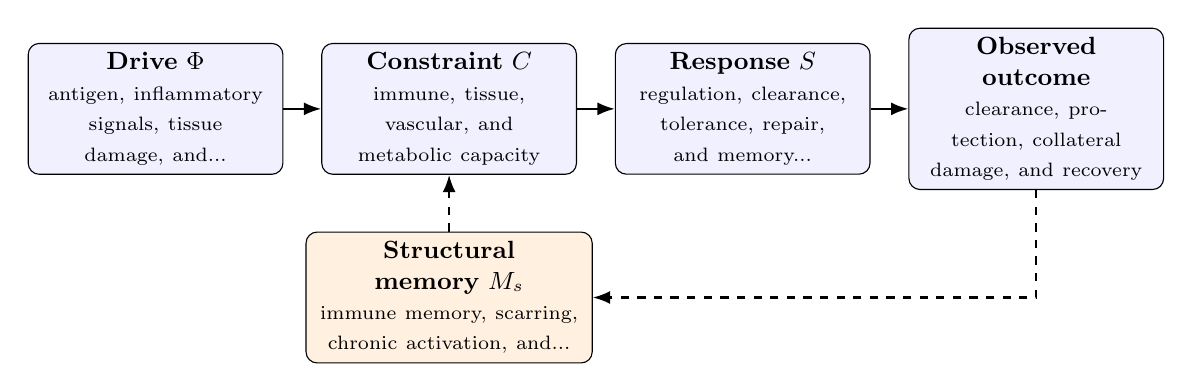
\begin{tikzpicture}[
    node distance=0.48cm,
    every node/.style={font=\small},
    box/.style={draw, rounded corners, align=center, minimum height=1.45cm, text width=3.0cm, fill=blue!6},
    memory/.style={draw, rounded corners, align=center, minimum height=1.25cm, text width=3.4cm, fill=orange!12},
    flow/.style={-{Latex[length=2.2mm]}, thick},
    feedback/.style={-{Latex[length=2.2mm]}, thick, dashed}
]
\node[box] (drive) {\textbf{Drive $\Phi$}\\\scriptsize antigen, inflammatory signals, tissue damage, and...};
\node[box, right=of drive] (constraint) {\textbf{Constraint $C$}\\\scriptsize immune, tissue, vascular, and metabolic capacity};
\node[box, right=of constraint] (response) {\textbf{Response $S$}\\\scriptsize regulation, clearance, tolerance, repair, and memory...};
\node[box, right=of response] (outcome) {\textbf{Observed outcome}\\\scriptsize clearance, protection, collateral damage, and recovery};
\node[memory, below=0.72cm of constraint] (memory) {\textbf{Structural memory $M_s$}\\\scriptsize immune memory, scarring, chronic activation, and...};
\draw[flow] (drive) -- (constraint);
\draw[flow] (constraint) -- (response);
\draw[flow] (response) -- (outcome);
\draw[feedback] (outcome.south) |- (memory.east);
\draw[feedback] (memory.north) -- (constraint.south);
\end{tikzpicture}
\caption{Paper D-12 observable CDFD/AFL architecture for Immune System. Solid arrows give the proposed forward chain; dashed arrows make history-dependent feedback explicit.}
\label{fig:d12-architecture}
\end{figure}

\subsection{Paper-Specific Causal Hypothesis}

For this paper, the hypothesized causal sequence is specific. A change in
antigen, inflammatory signals, tissue damage, and metabolic demand arrives faster than regulation, clearance, tolerance, repair, and memory response can compensate.
This raises or redistributes immune, tissue, vascular, and metabolic capacity. If the load persists,
the retained state encoded by immune memory, scarring, chronic activation, and exposure history changes the next response, so a later event of equal
magnitude can produce a different trajectory in clearance, protection, collateral damage, and recovery. The
scientific task is to estimate that sequence against the best ordinary model of
the domain, not merely to redescribe the outcome after it occurs.

\subsection{Cross-Scale Translation Without Mechanistic Erasure}

For the domain applications family, the cross-domain translation is a disciplined test across systems with very different material mechanisms. A valid mapping preserves the baseline science of the domain, declares the scale of every variable, and earns its place through a discriminating prediction rather than resemblance alone. \cite{Holling1973,Turing1952,Shannon1948,BakTangWiesenfeld1987}
The required scale declaration for this paper is seconds to lifetimes; molecules to organisms. At short
scales, the key question is whether the incoming drive is transmitted,
buffered, or diverted. At intermediate scales, response changes effective
capacity and network exposure. At long scales, retained structure can alter the
state space itself. A result is genuinely cross-scale only when the aggregation
rule is stated and the same conclusion is not an artifact of averaging.

\subsection{Evidence Ladder and Discriminating Tests}

\begin{table}[htbp]
\centering
\small
\caption{Evidence ladder for Paper D-12. Each rung can fail independently.}
\begin{tabularx}{\textwidth}{|p{0.17\textwidth}|X|X|}
\hline
\textbf{Test} & \textbf{Design} & \textbf{Discriminating result} \\
\hline
Proxy audit & Measure immune profiling, clinical trajectories, perturbation, pathology, and longitudinal cohorts and preregister how each record maps to $\Phi$, $C$, $S$, $M_s$, and $Y$. & The mapping fails if proxies are non-identifiable, circular, or change meaning across cases. \\
\hline
Load ramp & Apply or observe a repeated antigenic or inflammatory challenge while estimating the dominant constraint and response time. & A threshold claim requires a reproducible nonlinear change and uncertainty bounds, not a visually chosen breakpoint. \\
\hline
Recovery and memory & Match present load across units with different histories, then compare recovery paths. & The memory claim requires history-dependent divergence after current conditions are controlled. \\
\hline
Model comparison & Compare the baseline domain model with and without the CDFD/AFL state variables using held-out data. & The paper's stated falsifier is: history-sensitive terms do not improve protection or damage prediction beyond immunology baselines. \\
\hline
\end{tabularx}
\end{table}

\subsection{Research Programme and Boundary Conditions}

The immediate research programme has four steps. First, construct a documented
dataset from immune profiling, clinical trajectories, perturbation, pathology, and longitudinal cohorts and retain raw units before normalization.
Second, fit a baseline domain model and report its calibration and out-of-sample
error. Third, add the smallest identifiable CDFD/AFL state extension and test
whether it improves prediction of clearance, protection, collateral damage, and recovery. Fourth, repeat the
analysis across the declared scale range and publish negative cases as part of
the cross-domain translation audit.

% END PART IV MAJOR CROSS-DOMAIN UPGRADE

\section{Conclusion}
Immunology is fundamentally a study of thermodynamic constraint management. By treating the immune system through the lens of CDFD, we see that pathogens are simply competing flux networks, and immunity is the dynamic structural resistance deployed to maintain the host's topological integrity.
\section*{Conflict of Interest} The author declares no conflict of interest.
\section*{Data Availability}
Part-specific runtime diagnostics are under each Part's \path{outputs/} directory.

Release-wide code: \path{Part_E_Synthesis/supplementary/}.

Generated summaries: \path{Part_E_Synthesis/outputs/}.

Figures: \path{Part_E_Synthesis/figures/}.


\section{Reference Layer}
\bibliographystyle{plain}
\bibliography{universal_afl_references}
\end{document}
